\documentclass{article}
\linespread{1.25}

\usepackage[top = 1cm, right=2cm, left=2cm]{geometry}
\usepackage{graphicx}
\usepackage{xepersian}
\settextfont{B Nazanin}
\setlatinmonofont{CMU Serif}
%\setlatinmonofont{Times New Roman}
\setlatintextfont{Times New Roman}

% Set Latin Modern font for the bullets in itemizea
\newfontfamily\latinbullet{Latin Modern Roman}



\title{گزارش تکلیف 
	\lr{Analyzing Titanic Survival Rates}
}
\author{درس یادگیری ماشین}
\date{
	امیرحسین ابوالحسنی\\
	400405003
	}
	
	
% Commands
\newcommand{\column}[1]{\lr{\textit{#1}}}
\renewcommand{\labelitemi}{{\latinbullet\textbullet}} % Use the bullet from Latin Modern font

\begin{document}
	\maketitle
	
	\section*{مقدمه}
	تحلیل اکتشافی داده‌ها، یا
	\lr{Exploratory Data Analysis (EDA)}،
	به معنی بررسی داده‌ها به صورت آماری، پاکسازی داده ها و مصورسازی آنهاست، این کار یکی از مهمترین مراحل در یک پروژه علوم داده می‌باشد.\\
	در این گزارش، به تحلیل دیتاستی از مشخصات مسافران کشتی تایتانیک میپردازیم.
	\vspace{10pt}
	\section{بررسی معنایی دیتاست}
	دیتاست تایتانیک، متشکل از 11 ویژگی و 1309 نمونه می‌باشد.\\
	در اینجا معنی هریک از ستون‌ها ارائه می‌گردد:‌
	
	\begin{center}
		
			\begin{table}[!ht]
				\begin{tabular}{c|c|c}
					نگاشت & توضیح & ویژگی\\
					\hline
					\hline
					0 : مرده ، 1 : زنده& نجات یافتن & \column{Survived}\\
					1 : درجه یک ، 2 :‌ درجه دو ، 3 : درجه سه & نوع بلیط & \column{Pclass}\\
					0 : زن ، 1 : مرد & جنسیت & \column{Sex}\\
					& سن به سال،‌ برای کودکان زیر یک سال به صورت اعشاری می‌باشد. & \column{Age}\\
					& تعداد همسر، خواهر و برادر سوار بر کشتی & \column{SibSp}\\
					& نعداد والدین و فرزندان سوار بر کشتی & \column{ParCh}\\
					& شماره بلیط & \column{Ticket}\\
					& هزینه بلیط مسافر & \column{Fare}\\
					& شماره کابین & \column{Cabin}\\
					\lr{C = Cherbourg, Q = Queenstown, S = Southampton}
					& بندر محل سوار شدن & \column{Embarked}\\
				\end{tabular}
				\caption{توضیح ویژگی‌های دیتاست به همراه معنی هر مقدار}
			\end{table}	
	\end{center}
	\vspace{10pt}
	\section{جمع آوری و تمیز کردن دیتا}
	با توجه به اینکه ستون تارگت از فایل 
	\lr{test.csv}
	جدا شده و در فایل 
	\lr{gender submission.csv}
	قرار دارد، ابتدا با عملگر پیوند داخلی این دو دیتافریم را با با یکدیگر جوین می‌کنیم، دیتا فرم به دست آمده با 
	\lr{train.csv}
	کانکت شده و همه داده‌ها در یک دیتاست قرار می‌گیرند.\\
	در مرحله بعد ویژگی‌های 
	\column{Cabin, Ticket, Name}
	را از دیتاست حذف می‌کنیم، با این استدلال که این سه ستون ربطی به نجات یافتن و یا مرگ مسافر به صورت مستقیم ندارد.\\
	
	\subsection{مقادیر هیچ‌مقدار}
	همانطور که در شکل 
	\ref{fig: nullHist}
	و
	\ref{fig: nullpies}
	دیده می‌شود، در دیتاست ستون‌های 
	\column{Age, Fare, Embarked, Cabin}
	دارای مقادیر هیچ‌مقدار می‌باشند.\\
	\begin{figure}[!ht]
		\centering
		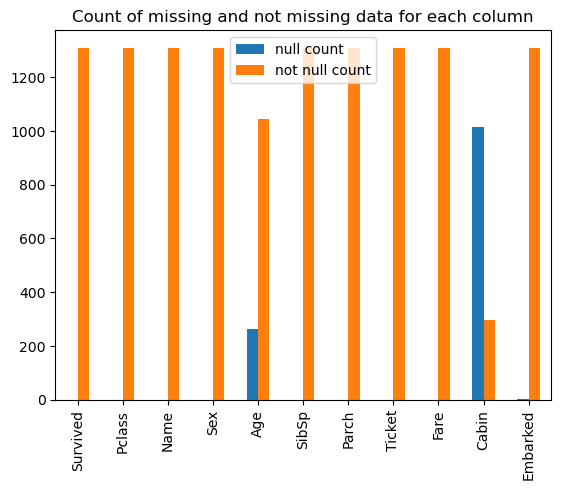
\includegraphics[scale=0.5]{./figs/Count-of-missing-and-not-missing data-for-each-column}
		\caption{
			فراوانی داده های هیج‌مقدار نسبت به داده‌های دارای مقدار برای هر ویژگی
		}
		\label{fig: nullHist}
	\end{figure}
	\begin{figure}[!ht]
		\centering
		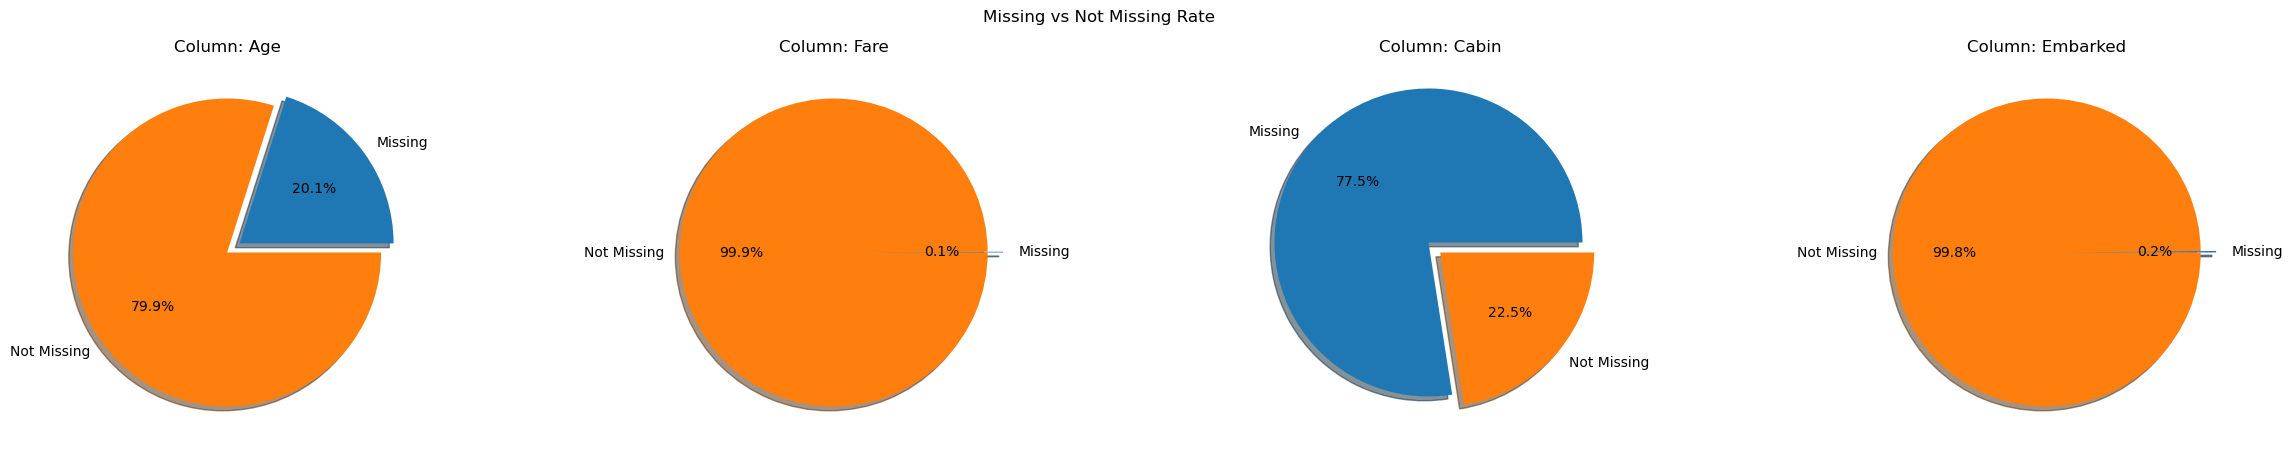
\includegraphics[scale=0.3]{./figs/Missing vs Not Missing Rate}
		\caption{
			نسبت داده‌های از دست داده شده به داده‌های موجود برای ستون‌های دارای مقادیر هیچ‌مقدار
		}
		\label{fig: nullpies}
	\end{figure}\\
	
	برای پر کردن، روش استفاده شده برای هر ستون به شرح زیر است:‌
	\begin{itemize}
		\item \column{Cabin}:
		این ستون در بخش قبل حذف شده است.
		
		\item \column{Fare}:‌
		از آنجایی که اثرگذارترین مشخصه ها در هزینه سفر، بدیهتا نوع بلیط و جنسیت می‌باشد و همچنین تعداد آن کم می‌باشد، داده ها را بر اساس این دو ویژگی گروه‌بندی کرده
		\footnote{
			معادل
			\lr{GroupBy}
			در
			\lr{SQL}
		}
		 و سپس میانگین هر گروه (که یکتا می‌باشد) را محاسبه می‌کنیم. حال با توجه به ترکیبی که ستون‌های 
		 \column{Pclass, Sex}
		 برای هر نمونه که دارای مقدار هیچ‌مقدار در ستون 
		 \column{Fare}
		 می‌باشد ایجاد می‌کند، میانگین مناسب خودش را در آن سلول میدهیم.
		 \begin{figure}[!ht]
		 	\centering
		 	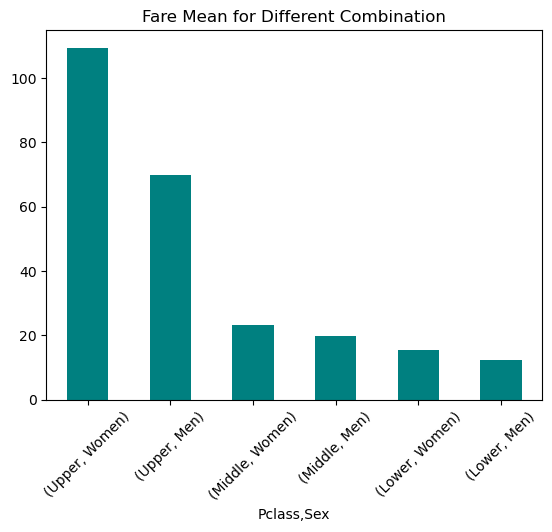
\includegraphics[scale=0.65]{./figs/Fare Mean for Different Combination}
		 	\caption{
		 		میانگین مقدار ویژگی 
		 		\column{Fare}
		 		برای ترکیب‌های یکتای 
		 		\column{Pclass, Sex}
		 	}
		 	\label{fig:FareMean}
		 \end{figure}
		 
		 \item \column{Embarked}: 
		 برای پر کردن بعضی سلول‌های ستون 
		 \column{Embarked}،
		 دیتاست بر اساس ستون
		 \column{Pclass}		 
		 گروه‌بندی شده و فروانی هر بندر در هر یک از این گروه ها محاسبه می‌شود. سپس بر اساس مقدار ستون 
		 \column{Pclass}		 
		 برای هر نمونه دارای هیچ‌مقدار در این ستون، بندری گذشته می‌شود که بیشتر مسافران آن نوع بلیط از آنجا سوار بر کشتی شده اند.
		 
		 \item \column{Age}:
		 برای این ستون که بیشترین مقدار هیچ‌مقدار را در بین ستون‌های موجود دارد، از متد 
		 \lr{Iterative Imputation}
		 استفاده شده است. این متد سعی بر این دارد که این ویژگی را به عنوان تابعی از ویژگی های دیگر در دیتاست ببیند و با برقراری ارتباط بین آن‌ها(به کمک رگرسیون) سعی بر تخمین مقادیر سن با توجه به دیگر ویژگی‌های هر نمونه دارد.
	\end{itemize}
	
	\newpage
	\section{آنالیزهای آماری و مصورسازی}\label{sec: stats}
	\subsection{جمعیت}
	 در اینجا مقدار تخصیص جمعیت به گروه ها‌ی مهم را مشاهده می‌کنیم.
	\begin{figure}[!ht]
		\centering
		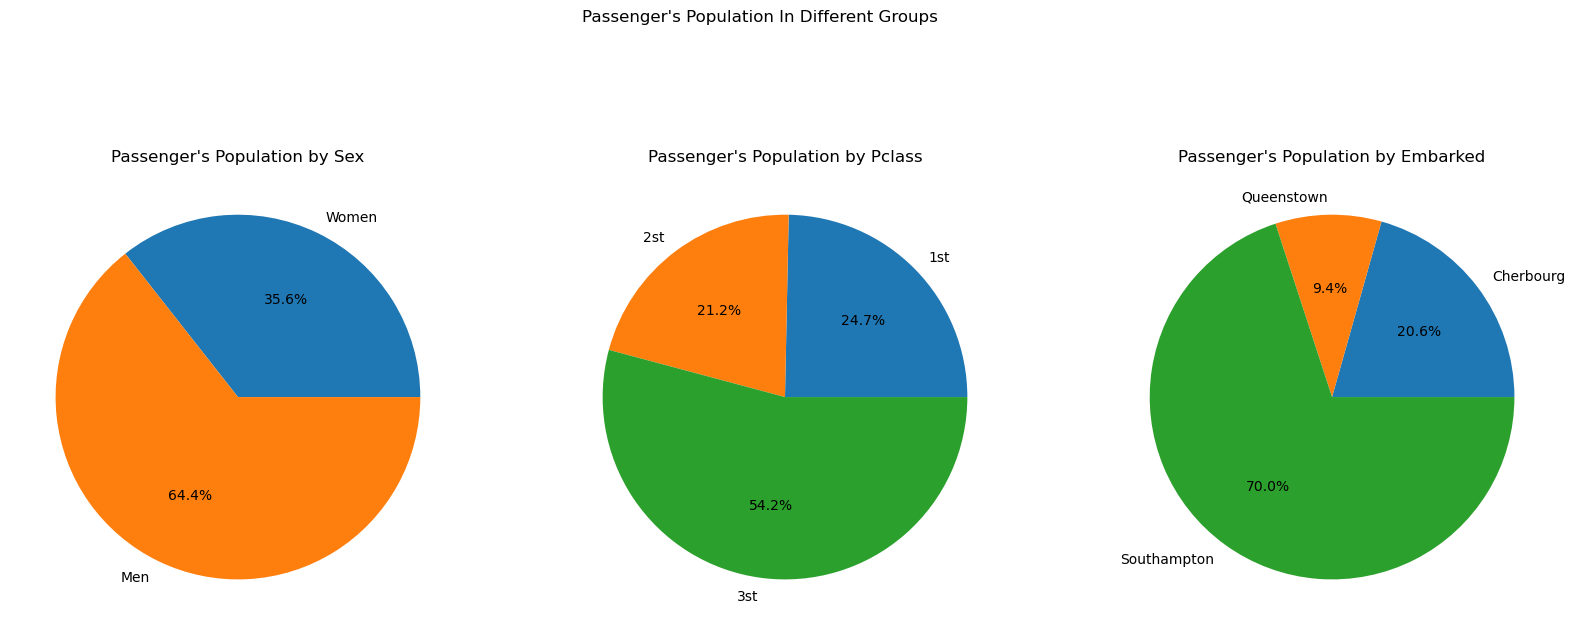
\includegraphics[scale=0.4]{./figs/Passenger's Population In Different Groups}
		\caption{
			نسبت پخش شدن جمعیت با توجه به ویژگی‌های 
			\column{Sex, Pclass, Embarked}
		}
		\label{fig: passenger's_Pop}
	\end{figure} 
	
	\subsection{نجات یافتگی}
	همانطور که از شکل 
	\ref{fig: SurvivalRatePie}
	پیداست،
	در این بخش بررسی می‌شود که در گروه‌های ویژگی‌های
	\column{Sex, Pclass}
	و در کل، فراوانی افراد نجات یافته و نیافته چگونه است.\\
	همچنین با این استدلال که پورت محل سوار شدن نباید تاثیری در زنده ماندن یا نماندن داشته باشد، از گروه بندی بر اساس این ستون صرف نظر شده است.\\
	\begin{figure}[h]
		\centering
		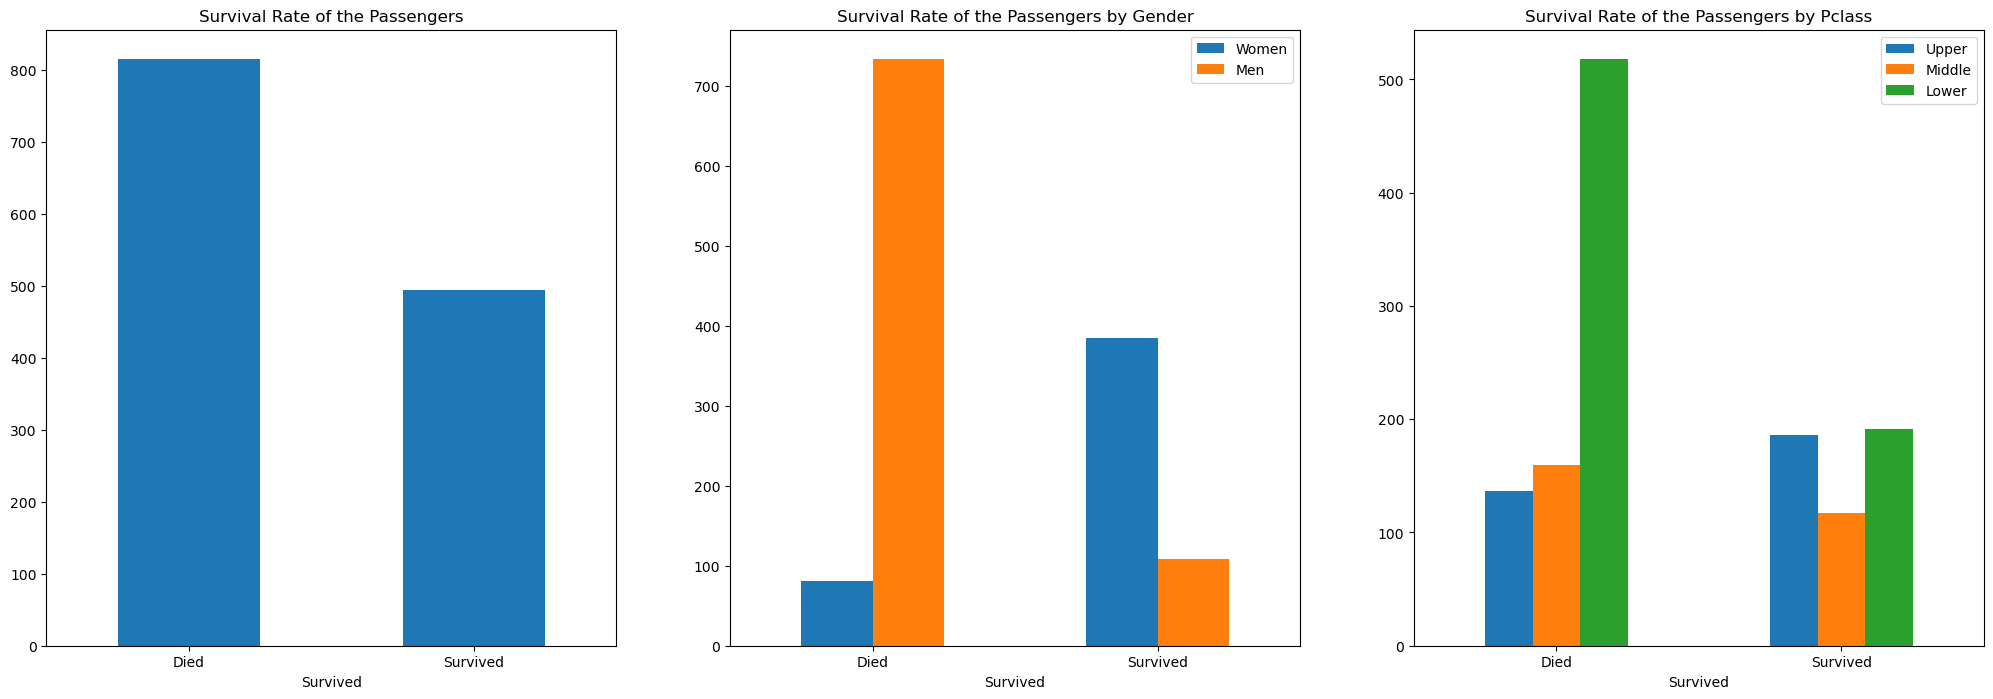
\includegraphics[scale=0.3]{./figs/Survival Rate of the Passengers by Pclass}
		\caption{
			نسبت پخش شدن نجات یافتگان و نیافتگان، با توجه به ویژگی‌های 
			\column{Sex, Pclass}
			و همچنین در تمامی نمونه‌ها
		}
		\label{fig: SurvivalRatePie}
	\end{figure}\\
	همانطور که در شکل 
	\ref{fig: SurvivalAgeDist}
	دیده می‌شود، در ادامه در گروه نجات یافته‌ها و نیافته‌ها، توزیع سن بررسی می‌شود تا کمک کند ترند‌های بین سن و وضعیت زنده ماندن را بیش از پیش متوجه شویم.
	\begin{figure}[h]
		\centering
		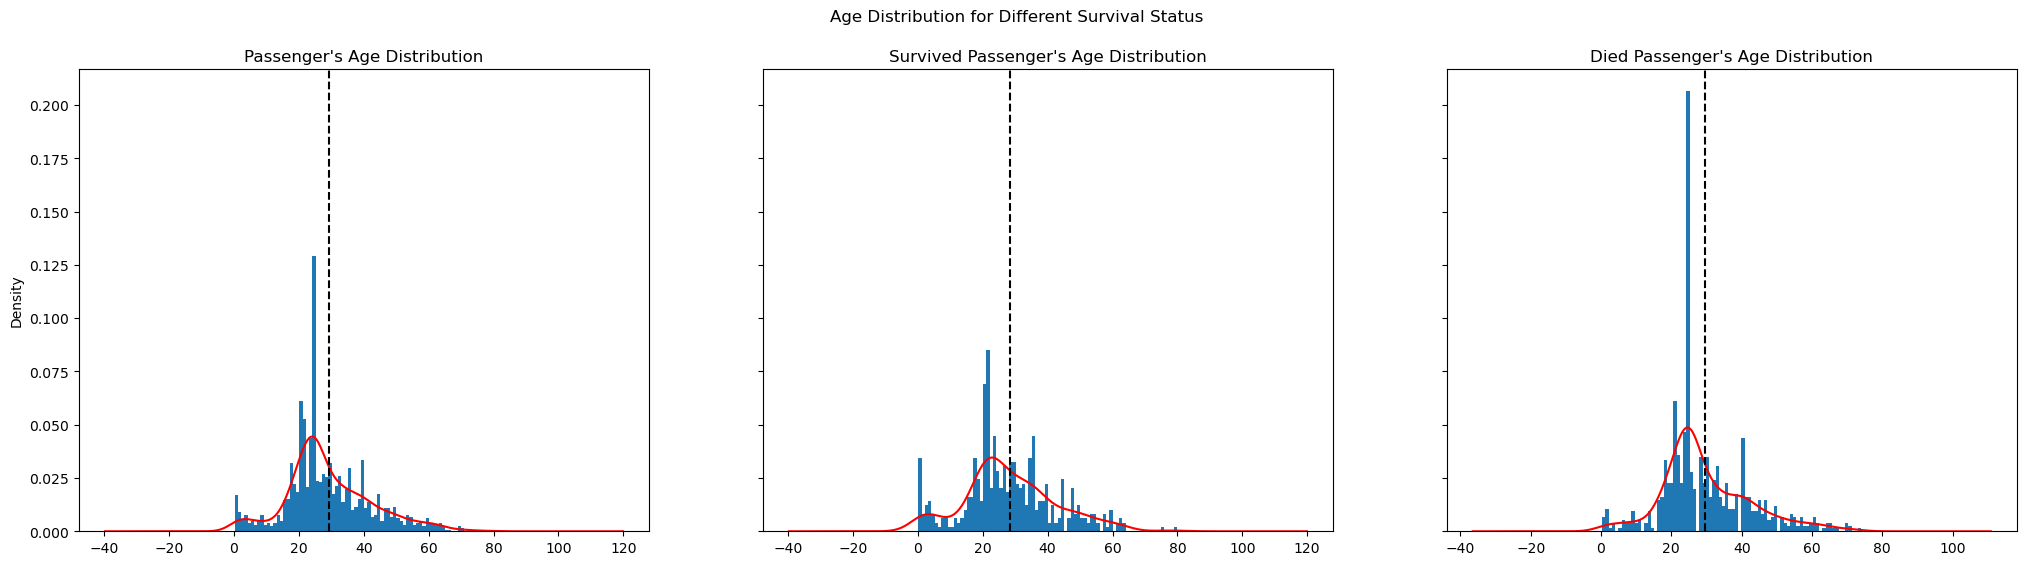
\includegraphics[scale=0.35]{./figs/Age Distribution for Different Survival Status}
		\caption{
			توزیع سن در گروه‌های ستون
			\column{Survived}
		}
		\label{fig: SurvivalAgeDist}
	\end{figure}\\
	می‌توان از ویژگی‌های 
	\column{SibSp, ParCh}
	برای متوجه شدن جمعیت نزدیکان هر مسافر استفاده کرده و رابطه این ویژگی جدید را با ویژگی نجات یافتگی به دست آورد.\\
	 برای این کار، این دو ستون با بکدیگر جمع شده و ستون جدیدی را به نام 
	 \column{Family Population}
	 ایجاد می‌کنند.
	\begin{figure}[!ht]
		\centering
		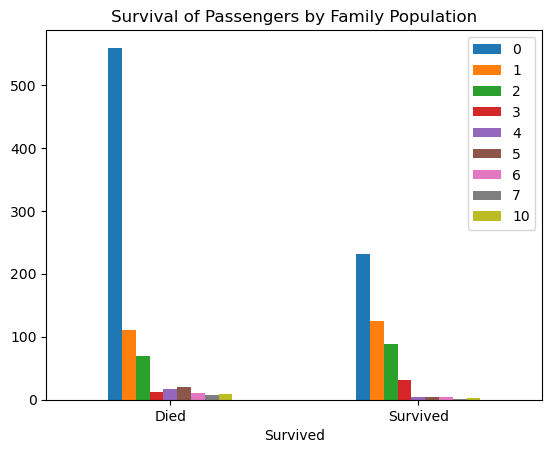
\includegraphics[scale=0.5]{./figs/Survival of Passengers by Family Population}
		\caption{
			فروانی جمعیت خانواده هر فرد در گروه‌های ستون
			\column{Survived}
		}
		\label{fig: Family Population}
	\end{figure} 
	
	\subsection{سن}
	پراکندگی داده‌ها با نمودار جعبه‌ای در این ویژگی بین کل مسافرین و همچنین بر اساس مقادیر ویژگی‌های 
	\column{Survived, Pclass}
	می‌تواند دید بهتری نسبت به داده‌ها به ما نشان دهد. (شکل~\ref{fig: AgeBoxPlot})
	
	\begin{figure}[!ht]
		\centering
		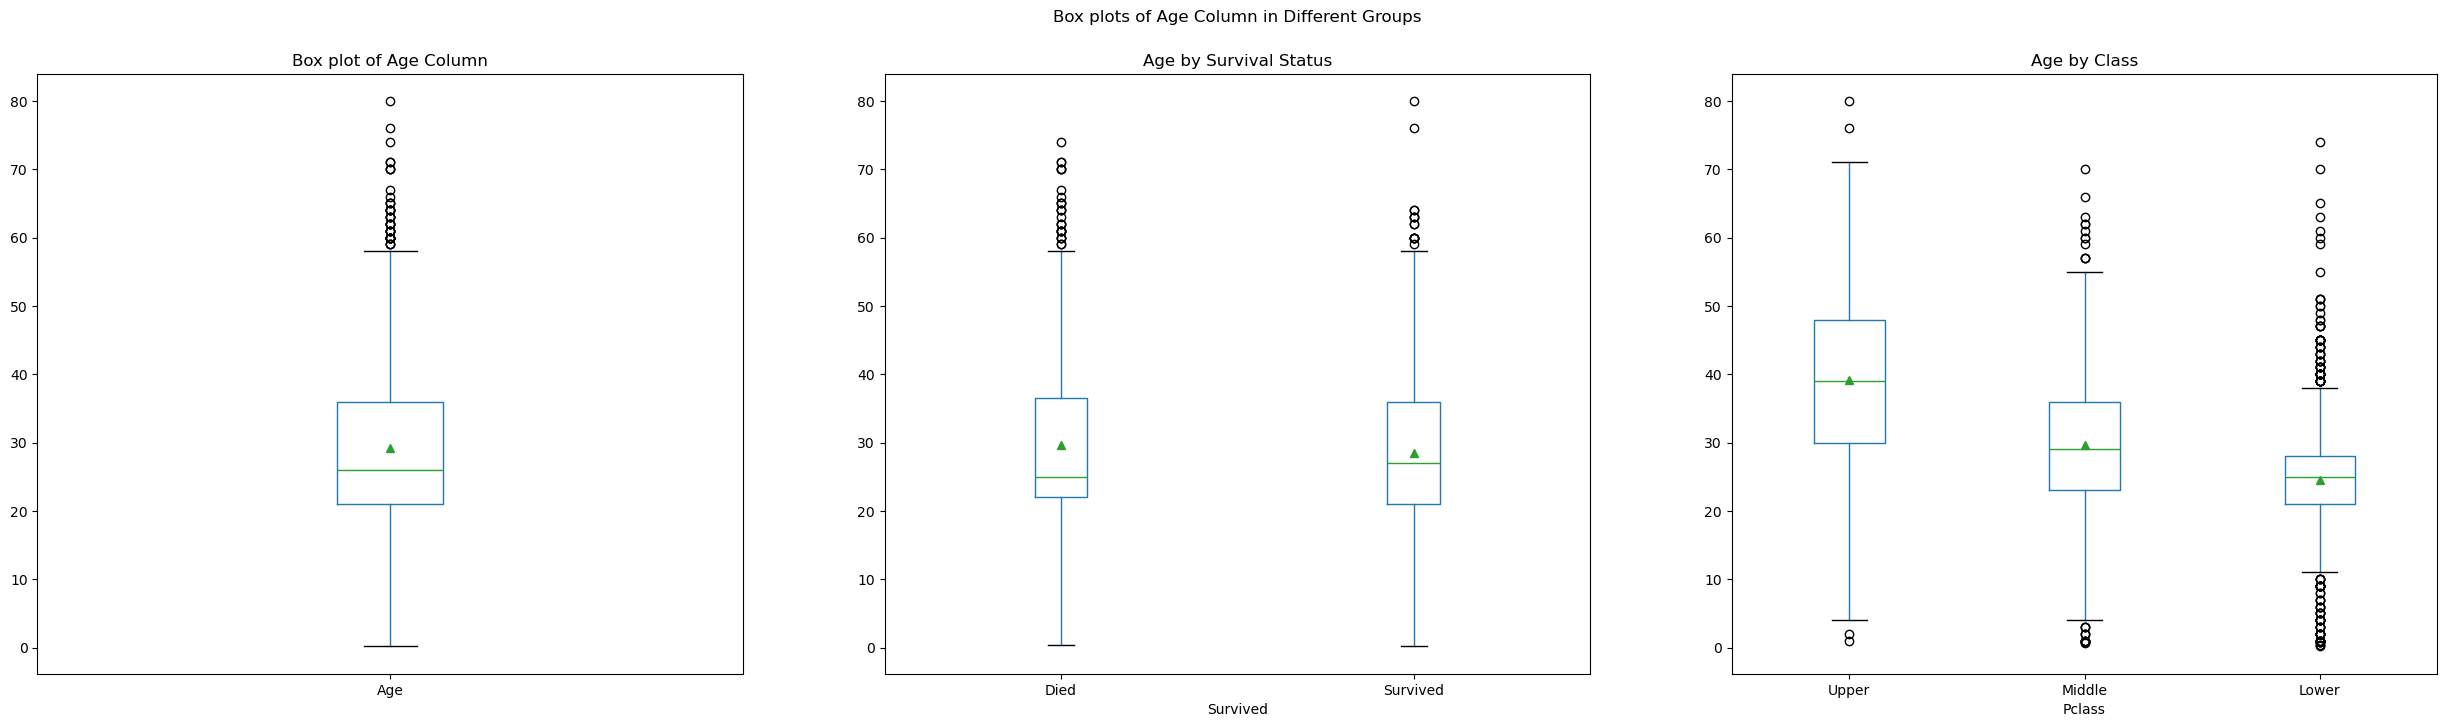
\includegraphics[scale=0.3]{./figs/Box plots of Age Column in Different Groups}
		\caption{
			نمودار جعبه‌ای برای ویژگی‌ سن با توجه به مقادیر ستون‌های
			\column{Survived, Pclass}
		}
		\label{fig: AgeBoxPlot}
	\end{figure}
	\vspace{10pt}
	
	\section*{نتیجه‌گیری}
	درباره ارتباطات بین ویژگی‌های دیتاست و زنده‌ماندن افراد، می‌توان با تکیه بر بخش 
	\ref{sec: stats}
	فرضیه‌هایی را اثبات کرد.
	
	در شکل 
	\ref{fig: SurvivalRatePie}
	می‌توان با نگاهی دقیق متوجه شد که بیش از نیمی از مسافران (حدود 800 نفر) جان خودشان را از دست داده اند که بیشترشان مرد بوده اند. این مورد با توجه به بیشتر بودن تعداد مردان نسبت به زنان 
	(شکل
	\ref{fig: passenger's_Pop}
	)
	 قابل استدلال می‌باشد.
	 
	 طبق شکل 
	 \ref{fig: Family Population}
	 جمعیت خوانواده هر مسافر بر روی کشتی، رابطه تقریبا معکوسی با زنده ماندن آن مسافر داشته است و این یکی از جالب ترین نکاتی‌ است که می‌توان در این آنالیزها به آن پی برد.
	 
	 از دیگر موارد بررسی شده این است که توزیع سن در گروه نجات یافته‌ها و نیافته‌ها چگونه است.\\
	 با توجه به شکل 
	 \ref{fig: SurvivalAgeDist}
	 و مقایسه رنج 0 تا 2 سال می‌توان فهمید که کودکان بسیار زیادی اللخصوص نوزادان زیر یک سال نجات داده شده اند.\\
	 توزیع بقیه سن‌ها در هر دو دسته تقریبا یکسان می‌باشد، تنها پیک در 25 سالگی افراد نجات نیافته پیداست  که با توجه به جمعیت بالای این دسته سنی 
	 (شکل 
	 \ref{fig: AgeBoxPlot})
	  بر روی کشتی قابل استدلال می‌باشد.
	  
	  پراکندگی سن با نمودارهای جعبه‌ای در شکل 
	  \ref{fig: AgeBoxPlot}
	  بسیار به ما در پیدا کردن میانگین و مد در گروه‌ها کمک می‌کند.
	  می‌توان برداشت کرد که افراد با سن بالای 60 سال بیشتر در دسته نجات نیافتگان حضور دارند. این مسئله را در شکل
	  \ref{fig: SurvivalAgeDist}
	  ~نیز می‌توان دید.\\
	  همچنین برای کلاس بلیط‌ها، می‌توان فهمید که عمده افراد طبقه 
	  \lr{Upper(1st)}
	  در اواخر دهه 30 خود به سر می‌بردند.\\
	  در طبقه متوسط، افراد در اواخر دهه 20 و در طبقه پایین، افراد در اواسط دهه 20 زندگی‌شان بودند.\\
	  برداشت دیگر از این شکل این است که بیشتر کودکان تا 15 سال از طبقه بالا و متوسط بودند، برای همین است که برای طبقه پایین داده نویز به شمار میروند.\\
	  همچنین افراد بالا 40 سال بیشتر مربوط به طبقه بالا و متوسط بوده اند. همانطور که دیده‌شد، این نمودار ارتباطات جالبی را در رابطه با سن افراد و کلاس سفر،‌و یا نجات یافتن نشان میدهد.
	  
	  \section*{منابع}
	  
	 \begin{enumerate}
	 	\item \lr{“Exploratory Data Analysis” Wikipedia.org}
	 	\item \lr{“Titanic - Machine Learning from Disaster”, Data Dictionary, Kaggle.com}
	 	\item \lr{“Handling missing values in dataset — 9 methods that you need to know”, medium.com}
	 \end{enumerate}
\end{document}